\documentclass {article}

 % Required for inserting code snippets
\usepackage{listings}
\usepackage{textcomp}
%\usepackage[spanish]{babel}
\usepackage[utf8x]{inputenc}
\usepackage{mathtools}
\usepackage{natbib}
\usepackage{floatrow}
\usepackage{verbatim}
\usepackage{graphicx}
\usepackage{caption}
\usepackage{subcaption}
\usepackage{url}
\usepackage{cancel}
\usepackage{amssymb}

\DeclarePairedDelimiter\abs{\lvert}{\rvert}

%%%%%%%%%%%%% PARAGRAPHS %%%%%%%%%%%%%%%%%
%No ident in new paragraph
\usepackage[parfill]{parskip}
%% Add a space of 1.5 lines between paragraphs
\parskip=1.1\baselineskip

%\usepackage{tgadventor}
%\renewcommand*\familydefault{\sfdefault} %% Only if the base font of the document is to be sans serif
%\usepackage[T1]{fontenc}
%\usepackage{lxfonts}
\usepackage{bookman}

\newcommand{\specialcell}[2][c]{%
  \begin{tabular}[#1]{@{}c@{}}#2\end{tabular}}

\usepackage{float}

\makeindex

\begin{document}

    %%%%%%%%\frontmatter%%%%%%%%%%
    \title{Reporte Final Silicon Photonics}
\author{Tatiana López Guevara}
\maketitle


    \tableofcontents

    %%%%%%%%%\mainmatter%%%%%%%%%%
    \chapter{Fourier Series}
	\label{ch:fs}

	The frequency spectrum is a complex-valued function of the frequency variable, 
and thus it is usually specified in terms of an amplitude spectrum and a phase spectrum 
\cite{kamen2000fundamentals}. The complex exponential form is given by:

\begin{equation}
\begin{aligned}
x(t) &= \displaystyle\sum_{- \infty}^{\infty} X_n e^{j n \omega_0 t} \\
X_n &= \displaystyle\int_{-T/2}^{T/2} x(t) e^{-j n \omega_0 t} \; dt 
\label{eq:c11}
\end{aligned}
\end{equation}

In the next exercises we will also be using the first and/or the second 
derivative of the previous expressions (\ref{eq:c1p11}), and therefore
we write them here explicitly:

\begin{equation}
\begin{aligned}
\dot{x}(t) &= \displaystyle\sum_{- \infty}^{\infty} j n \omega_0 X_n e^{j n \omega_0 t} \\
j n \omega_0 X_n &= \displaystyle\int_{-T/2}^{T/2} \dot{x}(t) e^{-j n \omega_0 t} \; dt 
\label{eq:c12}
\end{aligned}
\end{equation}

\begin{equation}
\begin{aligned}
\ddot{x}(t) &= \displaystyle\sum_{- \infty}^{\infty} - n^2 \omega_0^2 X_n e^{j n \omega_0 t} \\
-n^2 \omega_0^2 X_n &= \displaystyle\int_{-T/2}^{T/2} \dot{x}(t) e^{-j n \omega_0 t} \; dt 
\label{eq:c13}
\end{aligned}
\end{equation}


	For each signal, find the Fourier transform, $X(\omega)$, and then plot $|X(\omega)|$ 
(note, you may want to use MATLAB for the plot in 3.)

\section*{Problem 1}

\begin{figure}[H]
\caption*{}
\centering
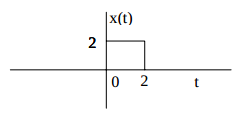
\includegraphics[width=0.4\textwidth]{figs/c2p11.png}
\label{fig:}
\end{figure} 

\subsection*{Solution}
Taking the derivative of $x(t)$ we get:

\begin{figure}[H]
\caption{Derivative $\dot{x}$}
\centering
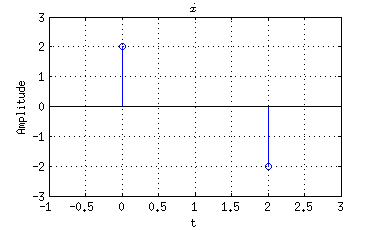
\includegraphics[width=0.6\textwidth]{figs/c2p1dotx.png}
\label{fig:}
\end{figure}

Applying \ref{eq:c21} and \ref{eq:c22c} to $\dot{x}$ we have:

\begin{equation*}
\begin{aligned}
j \omega X(\omega) &= 2 \int_{-\infty}^\infty (\delta(t) - \delta(t-2))e^{-j \omega t} \; dt\\
&= 2 [ 1 - e^{-2 j \omega}] \\
&= 2 e^{-j \omega}[ e^{- j \omega} - e^{- j \omega}] \\
&= 4 j e^{-j \omega} \sin(\omega) \\
X(\omega) &= 4 \frac{\sin(\omega) }{\omega} e^{-j \omega} \\
 &= 4 Sa(\omega) e^{- j \omega}
\end{aligned}
\end{equation*} 

The plot of the magintude and angle of $X(\omega)$ is:
\zcodemat{sources/c2p1a.m}{Plot of Magnitude and Angle}

\begin{figure}[H]
\caption{Magnitude $|X(\omega)|$ and Angle}
\centering
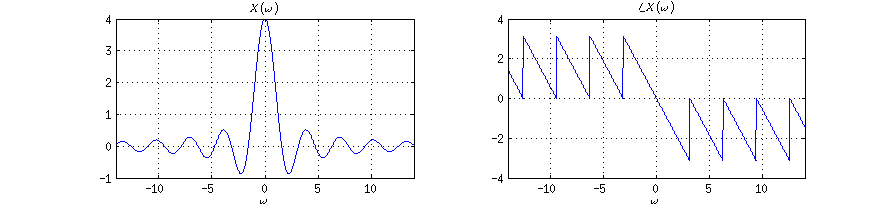
\includegraphics[width=1.0\textwidth]{figs/c2p1a.png}
\label{fig:c2p1a}
\end{figure} 


	\section*{Problem 2}
Repeat problem 1 for the following signal:

\begin{figure}[H]
\caption*{}
\centering
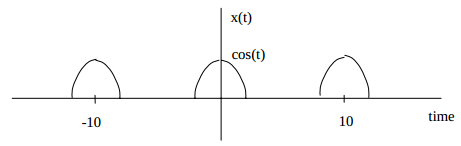
\includegraphics[width=0.8\textwidth]{figs/c1p2.png}
\label{fig:c1p2}
\end{figure} 

\subsection*{Solution}
The period of the shown signal is $T=10$ and therefore $\omega_0 = \frac{2 \pi}{T} =  \frac{\pi}{5}$.

If we take the first and second derivative of $x(t)$ we get:

\begin{figure}[H]
\caption{Derivative $\dot{x}$}
\centering
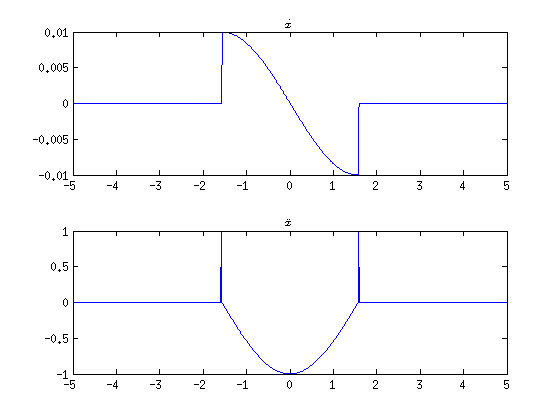
\includegraphics[width=0.8\textwidth]{figs/c1p2a.png}
\label{fig:c1p2a}
\end{figure} 

The range t = [-5,5] contains one complete period of the signal.
Applying (\ref{eq:c12}) we have:

\begin{equation*}
\begin{aligned}
\ddot{x}(t) &= - x(t) + \delta(t+\pi/2) + \delta(t-\pi/2)\\
\displaystyle\sum_{- \infty}^{\infty} - n^2 \omega_0^2 X_n e^{j n \omega_0 t} &=
\displaystyle\sum_{- \infty}^{\infty} X_n e^{j n \omega_0 t} + 
\delta(t+\pi/2) + \delta(t-\pi/2) \\
\displaystyle\sum_{- \infty}^{\infty} (1 - n^2 \omega_0^2) X_n e^{j n \omega_0 t} &=
\delta(t+\pi/2) + \delta(t-\pi/2) \\
\end{aligned}
\end{equation*} 

Whe can now obtain $X_n$ with:

\begin{equation*}
\begin{aligned}
(1 - n^2 \omega_0^2) X_n &= \frac{1}{T} \int_{-5}^5 \delta(t+\pi/2) + \delta(t-\pi/2) 
e^{-j n \omega_0 t} \; dt \\
&=\frac{1}{T} ( e^{j n \frac{\omega_0}{2}} + e^{- j n \frac{\omega_0}{2}} ) \\
X_n &= \frac{1}{5(1-\frac{n^2 \pi^2}{25})} \cos(\frac{n \pi^2}{10})
\end{aligned}
\end{equation*} 

Next we use Matlab to plot the magnitude and phase of the spectra using the script given in \cite{wprobl_c1}

\zcodemat{sources/c1p2.m}{Calculate and plot magnitude and phase of Xn}

\begin{figure}[H]
\caption{Magnitude and Angle $X_n$}
\centering
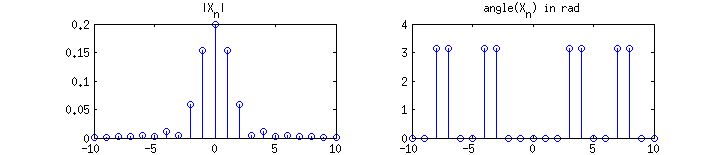
\includegraphics[width=0.8\textwidth]{figs/c1p2b.png}
\label{fig:c1p1b}
\end{figure} 

We then plot the approximation of the function using its Fourier coefficients 
\cite{wprobl_c1}.

\zcodemat{sources/fapprox2.m}{Approximation of x(t) with Fourier coefficients}

\begin{figure}[H]
\caption{Approximation of x(t) by Xn}
\centering
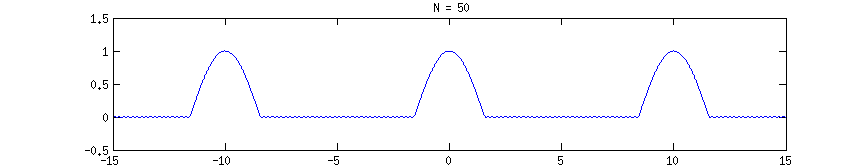
\includegraphics[width=0.8\textwidth]{figs/c1p2c.png}
\label{fig:c1p1c}
\end{figure} 

	\section*{Problem 3}

\begin{figure}[H]
\caption*{}
\centering
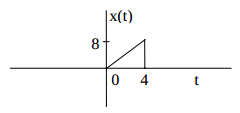
\includegraphics[width=0.4\textwidth]{figs/c2p3.png}
\label{fig:c2p3}
\end{figure} 

\subsection*{Solution}

Taking the derivative of $x(t)$ we get:

\begin{figure}[H]
\caption{Derivative $\dot{x}$}
\centering
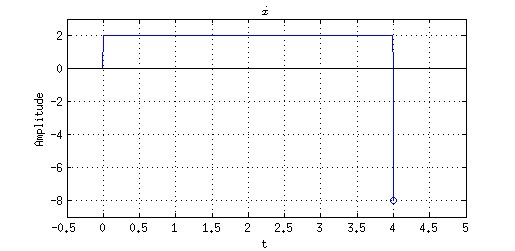
\includegraphics[width=0.6\textwidth]{figs/c2p3dotx.png}
\label{fig:c2p3dotx}
\end{figure}


Lets call $x_{p1}(t)$ and $X_{p1}(\omega)$ the function in time domain of the first point 
and its Fourier Transform respecively. 
We can express the first derivative of our function in terms of such function as:

\begin{equation*}
\dot{x}(t) = x_{p1}(t/2) - 8 \delta(t-4)
\end{equation*} 

As we can see from (\ref{eq:c22e}) the scale in time is reflected inversely
in the frecuency domain. 

\begin{equation*}
\begin{aligned}
j \omega X(\omega) &= X_{p1}(2 \omega) - 8 e^{-4 j \omega} \\
 &= 4 Sa(2 \omega) e^{- 2 j \omega}- 8e^{-4 j \omega} \\
X(\omega) &= \frac{4 j}{\omega} e^{-2 j \omega} [2 e^{-2 j \omega}- Sa(2 \omega)]
\end{aligned}
\end{equation*} 

The plot of the magintude and angle of $X(\omega)$ is:
\zcodemat{sources/c2p3a.m}{Plot of Magnitude and Angle}

\begin{figure}[H]
\caption{Magnitude $|X(\omega)|$ and Angle}
\centering
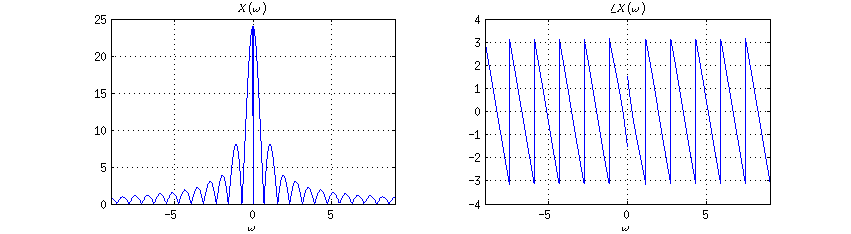
\includegraphics[width=1.0\textwidth]{figs/c2p3a.png}
\label{fig:c2p3a}
\end{figure} 


	\section*{Problem 4}

Repeat Problem 3 for $x(t) = 2 + \cos(50 \pi t)$ and T = 0.025 sec.

\begin{itemize}
\item  Draw $|X_s(\omega)|$ where $x_s(t) = x(t)p(t)$. Determine if aliasing occurs.
\end{itemize} 

\subsection*{Solution}

Since $T_s = 0.025 sec$ is greater than the minimum required,
aliasing will occur as can be seen in (\ref{fig:c3p4a}).

\begin{equation*}
\omega_s = \frac{2 \pi}{T_s} =  80 \pi
\end{equation*} 

\begin{figure}[H]
\caption{Sampling $|X_s(\omega)|$}
\centering
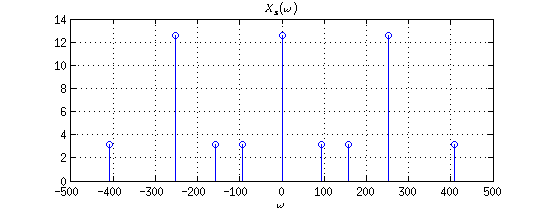
\includegraphics[width=0.8\textwidth]{figs/c3p4a.png}
\label{fig:c3p4a}
\end{figure}

\begin{itemize}
\item Determine the expression for y(t).
\end{itemize} 

\subsection*{Solution}

The limits of the lowpass filter are $-0.5 \omega_s = -40 \pi$ to $0.5 \omega_s = 40 \pi$.
The Fourier transform of $Y(\omega) = H(\omega)X(\omega)$ is:

\begin{figure}[H]
\caption{Magnitude $|X(\omega)|$}
\centering
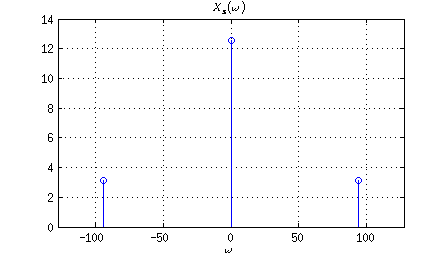
\includegraphics[width=0.6\textwidth]{figs/c3p4b.png}
\label{fig:c3p4b}
\end{figure}

And therefore:

\begin{equation*}
\begin{aligned}
y(t) = 2 + \cos(30 \pi t)
\end{aligned}
\end{equation*} 

\begin{itemize}
\item Determine an expression for x[n].
\end{itemize} 

\subsection*{Solution}

\begin{equation*}
\begin{aligned}
x(n) &= 2 + \cos(50 \pi n T_s) \\
     &= 2 + \cos(1.25 \pi n)
\end{aligned}
\end{equation*} 

	\section*{Problem 5}

Solve the following difference equation using z-transforms:

\begin{equation*}
\begin{aligned}
y[n] + 3y[n-1] + 2y[n-2] = 2x[n] - x[n-1]\\
y[-1] = 0\\
y[-2] = 1\\
\end{aligned}
\end{equation*} 

To the input:
\begin{equation*}
\begin{aligned}
x[n]=u[n]
\end{aligned}
\end{equation*} 

\subsection*{Solution}

\begin{equation*}
\begin{aligned}
y[z] + 3z^{-1}y[z] + 2(z^{-2}y[z]+1) &= 2\frac{z}{z-1} - \frac{1}{z-1}\\
y[z](z^2+3z+2) + 2z^2 &= 2 \frac{z^3}{z-1} - \frac{z^2}{z-1}\\
y[z] &= \frac{2z^3-z^2-2z^3+2z^2}{(z-1)(z+1)(z+2)} \\
&= \frac{z^2}{(z-1)(z+1)(z+2)} \\
\frac{y[z]}{z} &= \frac{z}{(z-1)(z+1)(z+2)} \\
&= \frac{A}{z-1} + \frac{B}{z+1} + \frac{C}{z+2}
\end{aligned}
\end{equation*} 

We find the values of $A,B,C$ using partial fractions:
\begin{equation*}
\begin{aligned}
A &= \frac{1}{6} \\
B &= \frac{1}{2} \\
C &= \frac{-2}{3}
\end{aligned}
\end{equation*} 

Therefore,
\begin{equation*}
\begin{aligned}
y[z] &= \frac{1}{6} \frac{z}{z-1} + \frac{1}{2} \frac{z}{z+1} - \frac{2}{3} \frac{z}{z+2} \\
y[n] &= \frac{1}{6} u[n] + \frac{1}{2} (-1)^n - \frac{2}{3} (-2)^n
\end{aligned}
\end{equation*} 

  

    \chapter{Fourier Transform}
    \label{ch:ft}
    The frequency spectrum is a complex-valued function of the frequency variable, 
and thus it is usually specified in terms of an amplitude spectrum and a phase spectrum 
\cite{kamen2000fundamentals}. The complex exponential form is given by:

\begin{equation}
\begin{aligned}
x(t) &= \displaystyle\sum_{- \infty}^{\infty} X_n e^{j n \omega_0 t} \\
X_n &= \displaystyle\int_{-T/2}^{T/2} x(t) e^{-j n \omega_0 t} \; dt 
\label{eq:c11}
\end{aligned}
\end{equation}

In the next exercises we will also be using the first and/or the second 
derivative of the previous expressions (\ref{eq:c1p11}), and therefore
we write them here explicitly:

\begin{equation}
\begin{aligned}
\dot{x}(t) &= \displaystyle\sum_{- \infty}^{\infty} j n \omega_0 X_n e^{j n \omega_0 t} \\
j n \omega_0 X_n &= \displaystyle\int_{-T/2}^{T/2} \dot{x}(t) e^{-j n \omega_0 t} \; dt 
\label{eq:c12}
\end{aligned}
\end{equation}

\begin{equation}
\begin{aligned}
\ddot{x}(t) &= \displaystyle\sum_{- \infty}^{\infty} - n^2 \omega_0^2 X_n e^{j n \omega_0 t} \\
-n^2 \omega_0^2 X_n &= \displaystyle\int_{-T/2}^{T/2} \dot{x}(t) e^{-j n \omega_0 t} \; dt 
\label{eq:c13}
\end{aligned}
\end{equation}


    For each signal, find the Fourier transform, $X(\omega)$, and then plot $|X(\omega)|$ 
(note, you may want to use MATLAB for the plot in 3.)

\section*{Problem 1}

\begin{figure}[H]
\caption*{}
\centering
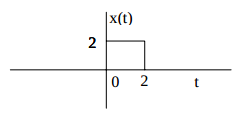
\includegraphics[width=0.4\textwidth]{figs/c2p11.png}
\label{fig:}
\end{figure} 

\subsection*{Solution}
Taking the derivative of $x(t)$ we get:

\begin{figure}[H]
\caption{Derivative $\dot{x}$}
\centering
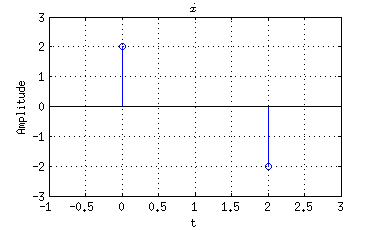
\includegraphics[width=0.6\textwidth]{figs/c2p1dotx.png}
\label{fig:}
\end{figure}

Applying \ref{eq:c21} and \ref{eq:c22c} to $\dot{x}$ we have:

\begin{equation*}
\begin{aligned}
j \omega X(\omega) &= 2 \int_{-\infty}^\infty (\delta(t) - \delta(t-2))e^{-j \omega t} \; dt\\
&= 2 [ 1 - e^{-2 j \omega}] \\
&= 2 e^{-j \omega}[ e^{- j \omega} - e^{- j \omega}] \\
&= 4 j e^{-j \omega} \sin(\omega) \\
X(\omega) &= 4 \frac{\sin(\omega) }{\omega} e^{-j \omega} \\
 &= 4 Sa(\omega) e^{- j \omega}
\end{aligned}
\end{equation*} 

The plot of the magintude and angle of $X(\omega)$ is:
\zcodemat{sources/c2p1a.m}{Plot of Magnitude and Angle}

\begin{figure}[H]
\caption{Magnitude $|X(\omega)|$ and Angle}
\centering
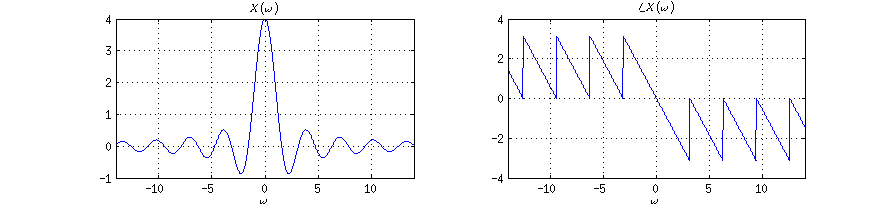
\includegraphics[width=1.0\textwidth]{figs/c2p1a.png}
\label{fig:c2p1a}
\end{figure} 


    \section*{Problem 2}
Repeat problem 1 for the following signal:

\begin{figure}[H]
\caption*{}
\centering
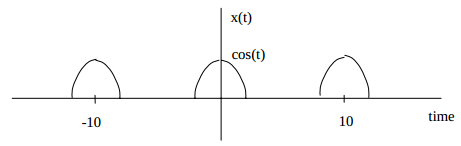
\includegraphics[width=0.8\textwidth]{figs/c1p2.png}
\label{fig:c1p2}
\end{figure} 

\subsection*{Solution}
The period of the shown signal is $T=10$ and therefore $\omega_0 = \frac{2 \pi}{T} =  \frac{\pi}{5}$.

If we take the first and second derivative of $x(t)$ we get:

\begin{figure}[H]
\caption{Derivative $\dot{x}$}
\centering
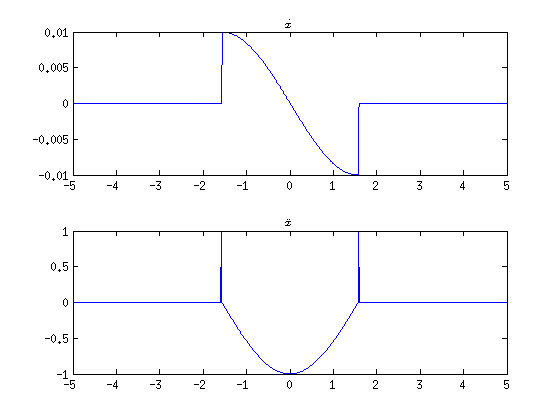
\includegraphics[width=0.8\textwidth]{figs/c1p2a.png}
\label{fig:c1p2a}
\end{figure} 

The range t = [-5,5] contains one complete period of the signal.
Applying (\ref{eq:c12}) we have:

\begin{equation*}
\begin{aligned}
\ddot{x}(t) &= - x(t) + \delta(t+\pi/2) + \delta(t-\pi/2)\\
\displaystyle\sum_{- \infty}^{\infty} - n^2 \omega_0^2 X_n e^{j n \omega_0 t} &=
\displaystyle\sum_{- \infty}^{\infty} X_n e^{j n \omega_0 t} + 
\delta(t+\pi/2) + \delta(t-\pi/2) \\
\displaystyle\sum_{- \infty}^{\infty} (1 - n^2 \omega_0^2) X_n e^{j n \omega_0 t} &=
\delta(t+\pi/2) + \delta(t-\pi/2) \\
\end{aligned}
\end{equation*} 

Whe can now obtain $X_n$ with:

\begin{equation*}
\begin{aligned}
(1 - n^2 \omega_0^2) X_n &= \frac{1}{T} \int_{-5}^5 \delta(t+\pi/2) + \delta(t-\pi/2) 
e^{-j n \omega_0 t} \; dt \\
&=\frac{1}{T} ( e^{j n \frac{\omega_0}{2}} + e^{- j n \frac{\omega_0}{2}} ) \\
X_n &= \frac{1}{5(1-\frac{n^2 \pi^2}{25})} \cos(\frac{n \pi^2}{10})
\end{aligned}
\end{equation*} 

Next we use Matlab to plot the magnitude and phase of the spectra using the script given in \cite{wprobl_c1}

\zcodemat{sources/c1p2.m}{Calculate and plot magnitude and phase of Xn}

\begin{figure}[H]
\caption{Magnitude and Angle $X_n$}
\centering
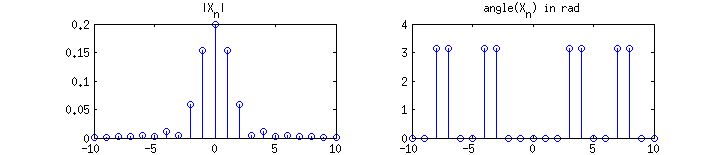
\includegraphics[width=0.8\textwidth]{figs/c1p2b.png}
\label{fig:c1p1b}
\end{figure} 

We then plot the approximation of the function using its Fourier coefficients 
\cite{wprobl_c1}.

\zcodemat{sources/fapprox2.m}{Approximation of x(t) with Fourier coefficients}

\begin{figure}[H]
\caption{Approximation of x(t) by Xn}
\centering
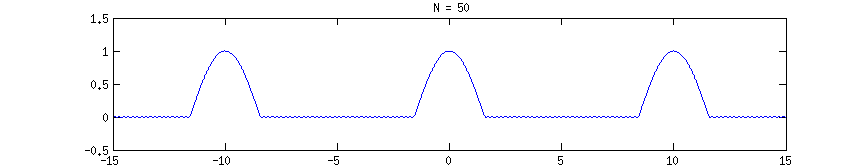
\includegraphics[width=0.8\textwidth]{figs/c1p2c.png}
\label{fig:c1p1c}
\end{figure} 

    \section*{Problem 3}

\begin{figure}[H]
\caption*{}
\centering
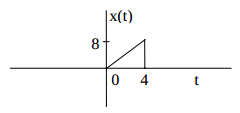
\includegraphics[width=0.4\textwidth]{figs/c2p3.png}
\label{fig:c2p3}
\end{figure} 

\subsection*{Solution}

Taking the derivative of $x(t)$ we get:

\begin{figure}[H]
\caption{Derivative $\dot{x}$}
\centering
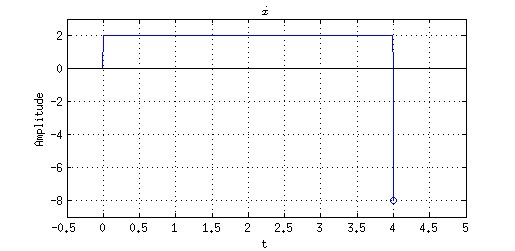
\includegraphics[width=0.6\textwidth]{figs/c2p3dotx.png}
\label{fig:c2p3dotx}
\end{figure}


Lets call $x_{p1}(t)$ and $X_{p1}(\omega)$ the function in time domain of the first point 
and its Fourier Transform respecively. 
We can express the first derivative of our function in terms of such function as:

\begin{equation*}
\dot{x}(t) = x_{p1}(t/2) - 8 \delta(t-4)
\end{equation*} 

As we can see from (\ref{eq:c22e}) the scale in time is reflected inversely
in the frecuency domain. 

\begin{equation*}
\begin{aligned}
j \omega X(\omega) &= X_{p1}(2 \omega) - 8 e^{-4 j \omega} \\
 &= 4 Sa(2 \omega) e^{- 2 j \omega}- 8e^{-4 j \omega} \\
X(\omega) &= \frac{4 j}{\omega} e^{-2 j \omega} [2 e^{-2 j \omega}- Sa(2 \omega)]
\end{aligned}
\end{equation*} 

The plot of the magintude and angle of $X(\omega)$ is:
\zcodemat{sources/c2p3a.m}{Plot of Magnitude and Angle}

\begin{figure}[H]
\caption{Magnitude $|X(\omega)|$ and Angle}
\centering
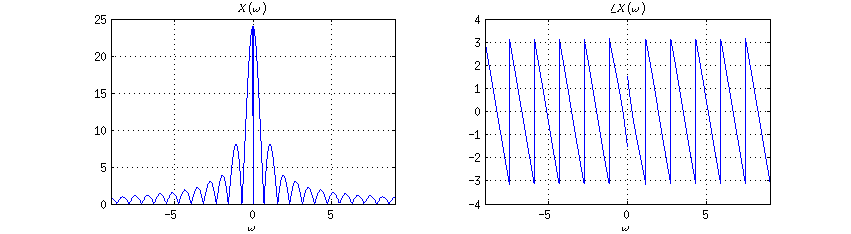
\includegraphics[width=1.0\textwidth]{figs/c2p3a.png}
\label{fig:c2p3a}
\end{figure} 


    \section*{Problem 4}

Repeat Problem 3 for $x(t) = 2 + \cos(50 \pi t)$ and T = 0.025 sec.

\begin{itemize}
\item  Draw $|X_s(\omega)|$ where $x_s(t) = x(t)p(t)$. Determine if aliasing occurs.
\end{itemize} 

\subsection*{Solution}

Since $T_s = 0.025 sec$ is greater than the minimum required,
aliasing will occur as can be seen in (\ref{fig:c3p4a}).

\begin{equation*}
\omega_s = \frac{2 \pi}{T_s} =  80 \pi
\end{equation*} 

\begin{figure}[H]
\caption{Sampling $|X_s(\omega)|$}
\centering
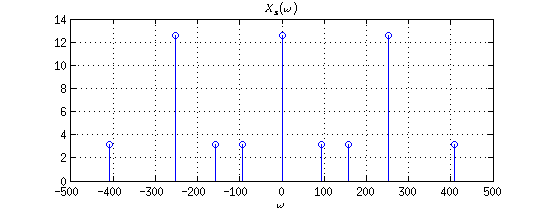
\includegraphics[width=0.8\textwidth]{figs/c3p4a.png}
\label{fig:c3p4a}
\end{figure}

\begin{itemize}
\item Determine the expression for y(t).
\end{itemize} 

\subsection*{Solution}

The limits of the lowpass filter are $-0.5 \omega_s = -40 \pi$ to $0.5 \omega_s = 40 \pi$.
The Fourier transform of $Y(\omega) = H(\omega)X(\omega)$ is:

\begin{figure}[H]
\caption{Magnitude $|X(\omega)|$}
\centering
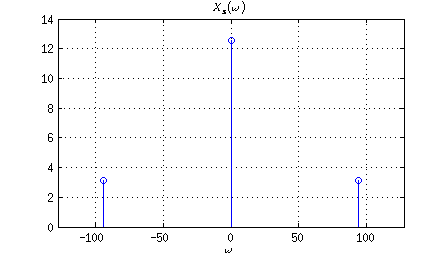
\includegraphics[width=0.6\textwidth]{figs/c3p4b.png}
\label{fig:c3p4b}
\end{figure}

And therefore:

\begin{equation*}
\begin{aligned}
y(t) = 2 + \cos(30 \pi t)
\end{aligned}
\end{equation*} 

\begin{itemize}
\item Determine an expression for x[n].
\end{itemize} 

\subsection*{Solution}

\begin{equation*}
\begin{aligned}
x(n) &= 2 + \cos(50 \pi n T_s) \\
     &= 2 + \cos(1.25 \pi n)
\end{aligned}
\end{equation*} 

    \section*{Problem 5}

Solve the following difference equation using z-transforms:

\begin{equation*}
\begin{aligned}
y[n] + 3y[n-1] + 2y[n-2] = 2x[n] - x[n-1]\\
y[-1] = 0\\
y[-2] = 1\\
\end{aligned}
\end{equation*} 

To the input:
\begin{equation*}
\begin{aligned}
x[n]=u[n]
\end{aligned}
\end{equation*} 

\subsection*{Solution}

\begin{equation*}
\begin{aligned}
y[z] + 3z^{-1}y[z] + 2(z^{-2}y[z]+1) &= 2\frac{z}{z-1} - \frac{1}{z-1}\\
y[z](z^2+3z+2) + 2z^2 &= 2 \frac{z^3}{z-1} - \frac{z^2}{z-1}\\
y[z] &= \frac{2z^3-z^2-2z^3+2z^2}{(z-1)(z+1)(z+2)} \\
&= \frac{z^2}{(z-1)(z+1)(z+2)} \\
\frac{y[z]}{z} &= \frac{z}{(z-1)(z+1)(z+2)} \\
&= \frac{A}{z-1} + \frac{B}{z+1} + \frac{C}{z+2}
\end{aligned}
\end{equation*} 

We find the values of $A,B,C$ using partial fractions:
\begin{equation*}
\begin{aligned}
A &= \frac{1}{6} \\
B &= \frac{1}{2} \\
C &= \frac{-2}{3}
\end{aligned}
\end{equation*} 

Therefore,
\begin{equation*}
\begin{aligned}
y[z] &= \frac{1}{6} \frac{z}{z-1} + \frac{1}{2} \frac{z}{z+1} - \frac{2}{3} \frac{z}{z+2} \\
y[n] &= \frac{1}{6} u[n] + \frac{1}{2} (-1)^n - \frac{2}{3} (-2)^n
\end{aligned}
\end{equation*} 

    \section*{Problem 6}

Consider the following sampling and reconstruction configuration:

\begin{figure}[H]
\caption*{}
\centering
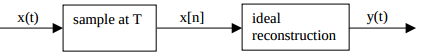
\includegraphics[width=0.7\textwidth]{figs/c3p31.png}
\label{fig:c3p31}
\end{figure} 

The output y(t) of the ideal reconstruction can be found by sending the sampled signal 
$x_s(t) = x(t)p(t)$ through an ideal lowpass filter:

\begin{figure}[H]
\caption*{}
\centering
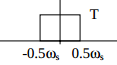
\includegraphics[width=0.2\textwidth]{figs/c3p32.png}
\label{fig:c3p32}
\end{figure} 

\begin{itemize}
\item Let $x(t) = 1 + cos(15\pi t)$ and T = 0.1 sec.
Draw $|X_s(\omega)|$ where $x_s(t) = x(t)p(t)$. 
Determine the expression for y(t).
\end{itemize} 

\subsection*{Solution}

First we calculate $X(\omega)$.

\begin{equation*}
\begin{aligned}
X(\omega) &= \pi [ 2 \delta(\omega) + 
	\delta(\omega - 15\pi) + \delta(\omega + 15 \pi)] 
\end{aligned}
\end{equation*} 

The plot of the magintude of $X(\omega)$ is:
\zcodemat{sources/c3p6a1.m}{Plot of Magnitude}

\begin{figure}[H]
\caption{Magnitude $|X(\omega)|$}
\centering
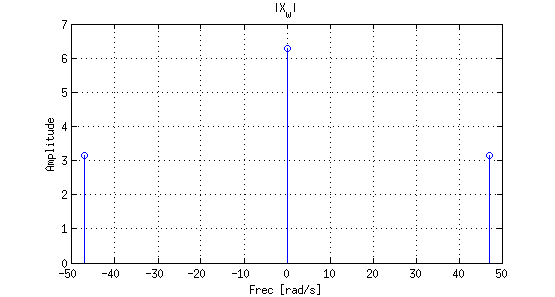
\includegraphics[width=0.8\textwidth]{figs/c3p6a1.png}
\label{fig:c3p6a1}
\end{figure} 

The minimum sampling period of the signal according to the Nyquist theorem is:

\begin{equation*}
\begin{aligned}
\omega_m &= 15 \pi \\
\omega_{Ns} >&= 2 \omega_m >= 30 \pi \\
T_{Ns} &= \frac{2 \pi}{\omega_s} <= \frac{1}{15} <= 0.066
\end{aligned}
\end{equation*} 

Since $T_s = 0.1 sec$ is greater than the minimum required,
aliasing will occur as can be seen in (\ref{fig:c3p6a2}).

\begin{equation*}
\omega_s = \frac{2 \pi}{T_s} =  20 \pi
\end{equation*} 

\zcodemat{sources/c3p6a2.m}{Plot of $|X_s(\omega)|$}

\begin{figure}[H]
\caption{Sampling $|X_s(\omega)|$}
\centering
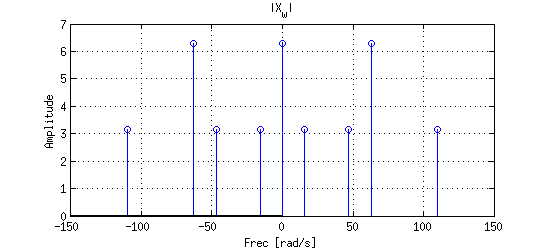
\includegraphics[width=0.8\textwidth]{figs/c3p6a2.png}
\label{fig:c3p6a2}
\end{figure}

The limits of the lowpass filter are $-0.5 \omega_s = -10 \pi$ to $0.5 \omega_s = 10 \pi$.
The Fourier transform of $Y(\omega) = H(\omega)X(\omega)$ is:

\begin{figure}[H]
\caption{Magnitude $|X(\omega)|$}
\centering
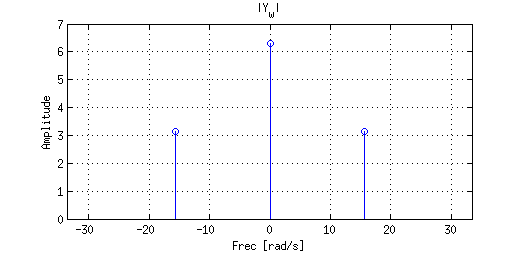
\includegraphics[width=0.8\textwidth]{figs/c3p6a3.png}
\label{fig:c3p6a3}
\end{figure}

And therefore only the $\omega = 5 \pi$ passes through it:

\begin{equation*}
\begin{aligned}
y(t) = 1 + cos(5 \pi t)
\end{aligned}
\end{equation*} 

%%%%%%%%%%%%%%%%%%%%%%%%%  B  %%%%%%%%%%%%%%%%%%%%%%%%%%%%
\begin{itemize}
\item Let $X(\omega) = \frac{1}{(j\omega+1)}$ and T = 1 sec.
Draw $|X_s(\omega)|$ where $x_s(t) = x(t)p(t)$. 
Does aliasing occur? (Justify your answer).
\end{itemize} 

\subsection*{Solution}

The magnitude of $X(\omega)$ is:
\begin{equation*}
\begin{aligned}
|X(\omega)| = \frac{1}{\omega^2 + 1}
\end{aligned}
\end{equation*} 

From the previous equation we can see that the function never intesects the w axis,
and therefore there will always be aliasing. 
However, setting $w_m$ to its FWHM we have:

\begin{equation*}
\begin{aligned}
\frac{1}{\omega_m^2+1} &= \frac{1}{2} \\
\omega_m = \sqrt{3}
\end{aligned}
\end{equation*} 

Hipoteticaly taking this value as $w_m$ we see that 
$w_s = 2 \pi > 2 w_m = 2 \sqrt{3} $ and in this case there will
not be aliasing.

The plot of the magintude of $X(\omega)$ and $X_s(\omega)$ is:
\zcodemat{sources/c3p6b1.m}{Plot of Magnitude}

\begin{figure}[H]
\caption{Magnitude}
\centering
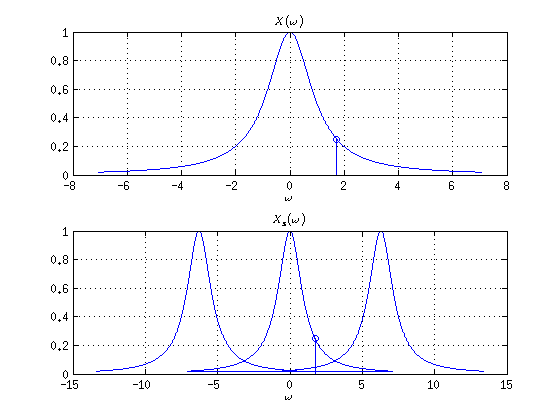
\includegraphics[width=0.8\textwidth]{figs/c3p6b2.png}
\label{fig:c3p6b2}
\end{figure} 


    \section*{Problem 7}

Use the FFT to approximate the Fourier Transform of $x(t) = 4e^{-t}u(t)$. 
Consider the following cases:

\begin{enumerate}
\item Sampling period T = 1, N = 10.
\item Sampling period T = 1, N = 20.
\item Sampling period T = 0.5, N = 20.
\item Sampling period T = 0.1, N = 100
\end{enumerate} 

\subsection*{Solution}

The fourier transform of $x(t)$ is:

\begin{equation*}
\begin{aligned}
X(\omega) = \frac{1}{1 +j \omega}
\end{aligned}
\end{equation*}

In order to approximate $X(\omega)$ using the $FFT$, the following
equation must be used \cite{kamen2000fundamentals}:

\begin{equation}
X(k\Gamma) = \frac{1 - e^{-j k \Gamma T}}{j k \Gamma} X_k
\label{eq:fftapprox}
\end{equation} 

Where $\Gamma = \frac{2\pi k}{N T}$ and $X_k$ is the output from the $FFT$ with $k=0,1,..,N-1$.

\zcodemat{sources/c4p7.m}{Mlab for plotting $X(\omega)$ and its approximation using $FFT$}

\begin{figure}[H]
\caption{Plot of $X(\omega)$ and approximation using $FFT$ for different $T$}
\centering
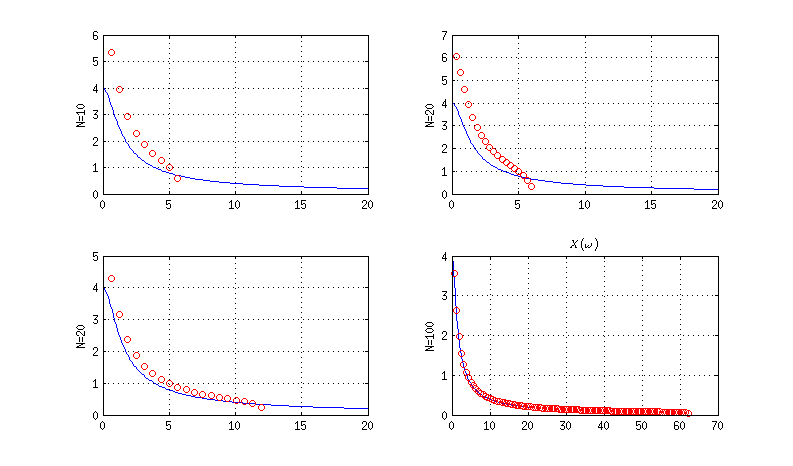
\includegraphics[width=0.8\textwidth]{figs/c4p7.png}
\label{fig:c4p7}
\end{figure}


    \section*{Problem 8}

Compute the inverse Fourier transform of the following signal

\begin{figure}[H]
\caption*{}
\centering
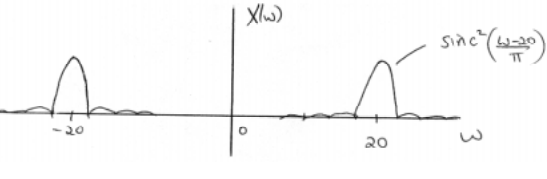
\includegraphics[width=0.8\textwidth]{figs/c2p8.png}
\label{fig:c2p8}
\end{figure} 

\subsection*{Solution}

From the 14th result of the Fourier Transforms table we have:

\begin{equation*}
Tr_\tau(t) =
\begin{cases}
	1 - \frac{|t|}{\tau}  ,& \mbox{if } |t| < \tau \\
	0                     ,& \mbox{if } |t| > \tau
\end{cases}
\end{equation*}

\begin{equation}
\begin{aligned}
\mathfrak{F}\{Tr_\tau(t)\} = \tau \left[ Sa \left( \frac{\omega \tau}{2} \right) \right]^2 \\
\mathfrak{F}\{Tr_2(t)\} = 2 Sa(\omega)^2 
\label{eq:c2p5}
\end{aligned}
\end{equation} 

First, we transform sinc into a known function like Sa: 
\begin{equation*}
\begin{aligned}
sinc^2 \left( \frac{\omega}{\pi} \right) = Sa^2(\omega)
\end{aligned}
\end{equation*} 

As we saw in Point 4, when we multiply by a $\cos$ in time 
we are adding 2 components of the function displaced simetrically
with half of its amplitude. The displacement in the plot is
of 20, therefore we need to multiply by a $\cos(20t)$.
We end up having:

\begin{equation*}
x(t) = Tr_2(t) \cos(20t)
\end{equation*} 


    \chapter{Sampling and Reconstruction}
    \label{ch:sr}
    For each signal, find the Fourier transform, $X(\omega)$, and then plot $|X(\omega)|$ 
(note, you may want to use MATLAB for the plot in 3.)

\section*{Problem 1}

\begin{figure}[H]
\caption*{}
\centering
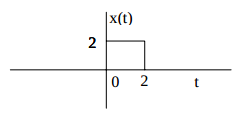
\includegraphics[width=0.4\textwidth]{figs/c2p11.png}
\label{fig:}
\end{figure} 

\subsection*{Solution}
Taking the derivative of $x(t)$ we get:

\begin{figure}[H]
\caption{Derivative $\dot{x}$}
\centering
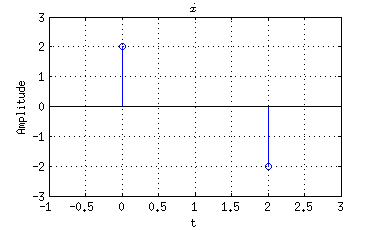
\includegraphics[width=0.6\textwidth]{figs/c2p1dotx.png}
\label{fig:}
\end{figure}

Applying \ref{eq:c21} and \ref{eq:c22c} to $\dot{x}$ we have:

\begin{equation*}
\begin{aligned}
j \omega X(\omega) &= 2 \int_{-\infty}^\infty (\delta(t) - \delta(t-2))e^{-j \omega t} \; dt\\
&= 2 [ 1 - e^{-2 j \omega}] \\
&= 2 e^{-j \omega}[ e^{- j \omega} - e^{- j \omega}] \\
&= 4 j e^{-j \omega} \sin(\omega) \\
X(\omega) &= 4 \frac{\sin(\omega) }{\omega} e^{-j \omega} \\
 &= 4 Sa(\omega) e^{- j \omega}
\end{aligned}
\end{equation*} 

The plot of the magintude and angle of $X(\omega)$ is:
\zcodemat{sources/c2p1a.m}{Plot of Magnitude and Angle}

\begin{figure}[H]
\caption{Magnitude $|X(\omega)|$ and Angle}
\centering
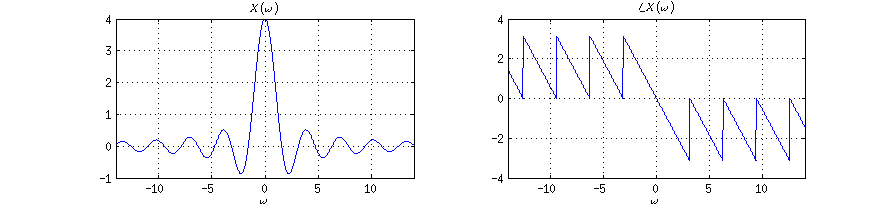
\includegraphics[width=1.0\textwidth]{figs/c2p1a.png}
\label{fig:c2p1a}
\end{figure} 


    \section*{Problem 2}
Repeat problem 1 for the following signal:

\begin{figure}[H]
\caption*{}
\centering
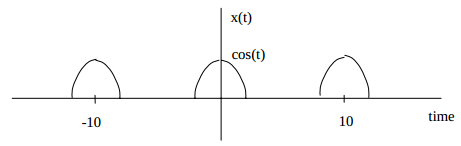
\includegraphics[width=0.8\textwidth]{figs/c1p2.png}
\label{fig:c1p2}
\end{figure} 

\subsection*{Solution}
The period of the shown signal is $T=10$ and therefore $\omega_0 = \frac{2 \pi}{T} =  \frac{\pi}{5}$.

If we take the first and second derivative of $x(t)$ we get:

\begin{figure}[H]
\caption{Derivative $\dot{x}$}
\centering
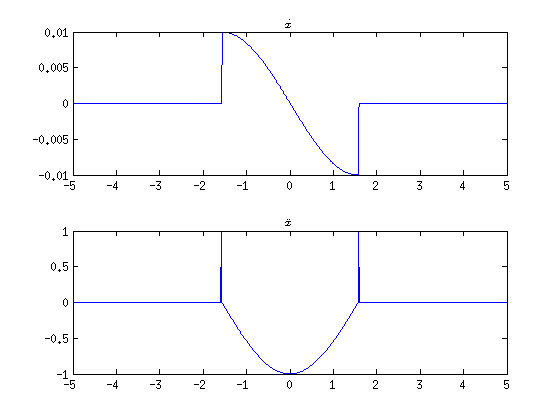
\includegraphics[width=0.8\textwidth]{figs/c1p2a.png}
\label{fig:c1p2a}
\end{figure} 

The range t = [-5,5] contains one complete period of the signal.
Applying (\ref{eq:c12}) we have:

\begin{equation*}
\begin{aligned}
\ddot{x}(t) &= - x(t) + \delta(t+\pi/2) + \delta(t-\pi/2)\\
\displaystyle\sum_{- \infty}^{\infty} - n^2 \omega_0^2 X_n e^{j n \omega_0 t} &=
\displaystyle\sum_{- \infty}^{\infty} X_n e^{j n \omega_0 t} + 
\delta(t+\pi/2) + \delta(t-\pi/2) \\
\displaystyle\sum_{- \infty}^{\infty} (1 - n^2 \omega_0^2) X_n e^{j n \omega_0 t} &=
\delta(t+\pi/2) + \delta(t-\pi/2) \\
\end{aligned}
\end{equation*} 

Whe can now obtain $X_n$ with:

\begin{equation*}
\begin{aligned}
(1 - n^2 \omega_0^2) X_n &= \frac{1}{T} \int_{-5}^5 \delta(t+\pi/2) + \delta(t-\pi/2) 
e^{-j n \omega_0 t} \; dt \\
&=\frac{1}{T} ( e^{j n \frac{\omega_0}{2}} + e^{- j n \frac{\omega_0}{2}} ) \\
X_n &= \frac{1}{5(1-\frac{n^2 \pi^2}{25})} \cos(\frac{n \pi^2}{10})
\end{aligned}
\end{equation*} 

Next we use Matlab to plot the magnitude and phase of the spectra using the script given in \cite{wprobl_c1}

\zcodemat{sources/c1p2.m}{Calculate and plot magnitude and phase of Xn}

\begin{figure}[H]
\caption{Magnitude and Angle $X_n$}
\centering
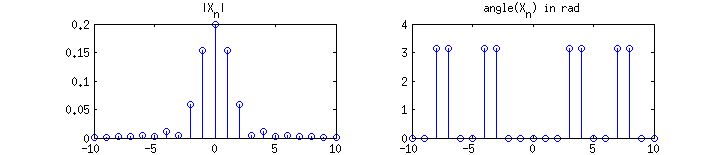
\includegraphics[width=0.8\textwidth]{figs/c1p2b.png}
\label{fig:c1p1b}
\end{figure} 

We then plot the approximation of the function using its Fourier coefficients 
\cite{wprobl_c1}.

\zcodemat{sources/fapprox2.m}{Approximation of x(t) with Fourier coefficients}

\begin{figure}[H]
\caption{Approximation of x(t) by Xn}
\centering
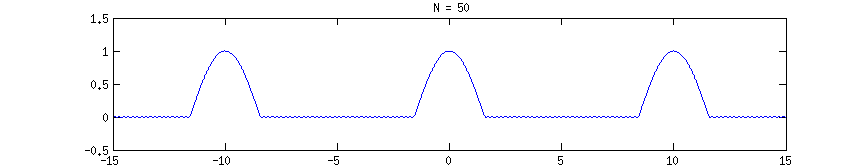
\includegraphics[width=0.8\textwidth]{figs/c1p2c.png}
\label{fig:c1p1c}
\end{figure} 

    \section*{Problem 3}

\begin{figure}[H]
\caption*{}
\centering
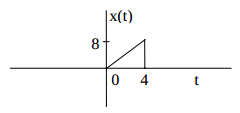
\includegraphics[width=0.4\textwidth]{figs/c2p3.png}
\label{fig:c2p3}
\end{figure} 

\subsection*{Solution}

Taking the derivative of $x(t)$ we get:

\begin{figure}[H]
\caption{Derivative $\dot{x}$}
\centering
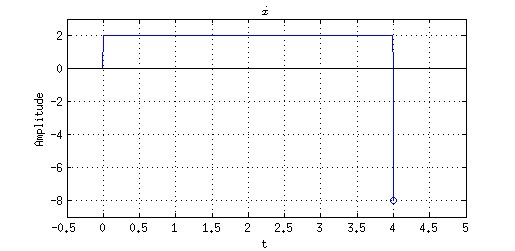
\includegraphics[width=0.6\textwidth]{figs/c2p3dotx.png}
\label{fig:c2p3dotx}
\end{figure}


Lets call $x_{p1}(t)$ and $X_{p1}(\omega)$ the function in time domain of the first point 
and its Fourier Transform respecively. 
We can express the first derivative of our function in terms of such function as:

\begin{equation*}
\dot{x}(t) = x_{p1}(t/2) - 8 \delta(t-4)
\end{equation*} 

As we can see from (\ref{eq:c22e}) the scale in time is reflected inversely
in the frecuency domain. 

\begin{equation*}
\begin{aligned}
j \omega X(\omega) &= X_{p1}(2 \omega) - 8 e^{-4 j \omega} \\
 &= 4 Sa(2 \omega) e^{- 2 j \omega}- 8e^{-4 j \omega} \\
X(\omega) &= \frac{4 j}{\omega} e^{-2 j \omega} [2 e^{-2 j \omega}- Sa(2 \omega)]
\end{aligned}
\end{equation*} 

The plot of the magintude and angle of $X(\omega)$ is:
\zcodemat{sources/c2p3a.m}{Plot of Magnitude and Angle}

\begin{figure}[H]
\caption{Magnitude $|X(\omega)|$ and Angle}
\centering
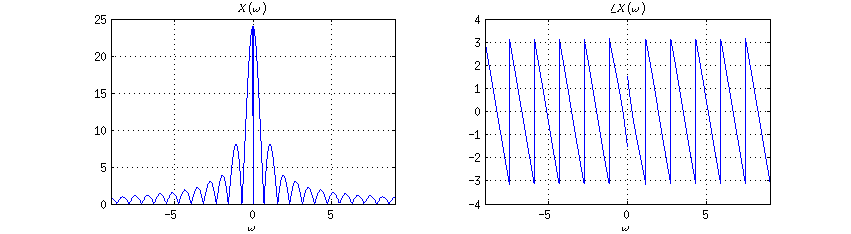
\includegraphics[width=1.0\textwidth]{figs/c2p3a.png}
\label{fig:c2p3a}
\end{figure} 


    \section*{Problem 4}

Repeat Problem 3 for $x(t) = 2 + \cos(50 \pi t)$ and T = 0.025 sec.

\begin{itemize}
\item  Draw $|X_s(\omega)|$ where $x_s(t) = x(t)p(t)$. Determine if aliasing occurs.
\end{itemize} 

\subsection*{Solution}

Since $T_s = 0.025 sec$ is greater than the minimum required,
aliasing will occur as can be seen in (\ref{fig:c3p4a}).

\begin{equation*}
\omega_s = \frac{2 \pi}{T_s} =  80 \pi
\end{equation*} 

\begin{figure}[H]
\caption{Sampling $|X_s(\omega)|$}
\centering
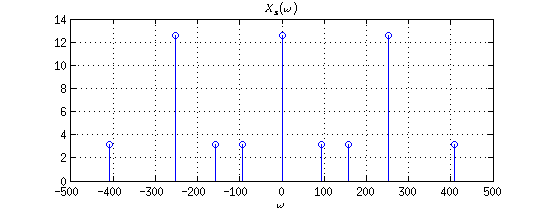
\includegraphics[width=0.8\textwidth]{figs/c3p4a.png}
\label{fig:c3p4a}
\end{figure}

\begin{itemize}
\item Determine the expression for y(t).
\end{itemize} 

\subsection*{Solution}

The limits of the lowpass filter are $-0.5 \omega_s = -40 \pi$ to $0.5 \omega_s = 40 \pi$.
The Fourier transform of $Y(\omega) = H(\omega)X(\omega)$ is:

\begin{figure}[H]
\caption{Magnitude $|X(\omega)|$}
\centering
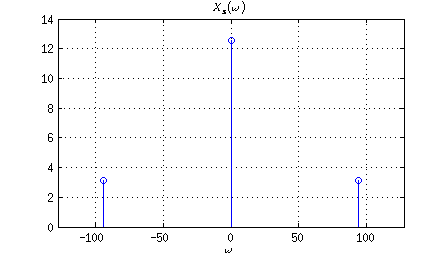
\includegraphics[width=0.6\textwidth]{figs/c3p4b.png}
\label{fig:c3p4b}
\end{figure}

And therefore:

\begin{equation*}
\begin{aligned}
y(t) = 2 + \cos(30 \pi t)
\end{aligned}
\end{equation*} 

\begin{itemize}
\item Determine an expression for x[n].
\end{itemize} 

\subsection*{Solution}

\begin{equation*}
\begin{aligned}
x(n) &= 2 + \cos(50 \pi n T_s) \\
     &= 2 + \cos(1.25 \pi n)
\end{aligned}
\end{equation*} 

    \section*{Problem 5}

Solve the following difference equation using z-transforms:

\begin{equation*}
\begin{aligned}
y[n] + 3y[n-1] + 2y[n-2] = 2x[n] - x[n-1]\\
y[-1] = 0\\
y[-2] = 1\\
\end{aligned}
\end{equation*} 

To the input:
\begin{equation*}
\begin{aligned}
x[n]=u[n]
\end{aligned}
\end{equation*} 

\subsection*{Solution}

\begin{equation*}
\begin{aligned}
y[z] + 3z^{-1}y[z] + 2(z^{-2}y[z]+1) &= 2\frac{z}{z-1} - \frac{1}{z-1}\\
y[z](z^2+3z+2) + 2z^2 &= 2 \frac{z^3}{z-1} - \frac{z^2}{z-1}\\
y[z] &= \frac{2z^3-z^2-2z^3+2z^2}{(z-1)(z+1)(z+2)} \\
&= \frac{z^2}{(z-1)(z+1)(z+2)} \\
\frac{y[z]}{z} &= \frac{z}{(z-1)(z+1)(z+2)} \\
&= \frac{A}{z-1} + \frac{B}{z+1} + \frac{C}{z+2}
\end{aligned}
\end{equation*} 

We find the values of $A,B,C$ using partial fractions:
\begin{equation*}
\begin{aligned}
A &= \frac{1}{6} \\
B &= \frac{1}{2} \\
C &= \frac{-2}{3}
\end{aligned}
\end{equation*} 

Therefore,
\begin{equation*}
\begin{aligned}
y[z] &= \frac{1}{6} \frac{z}{z-1} + \frac{1}{2} \frac{z}{z+1} - \frac{2}{3} \frac{z}{z+2} \\
y[n] &= \frac{1}{6} u[n] + \frac{1}{2} (-1)^n - \frac{2}{3} (-2)^n
\end{aligned}
\end{equation*} 

    \section*{Problem 6}

Consider the following sampling and reconstruction configuration:

\begin{figure}[H]
\caption*{}
\centering
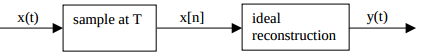
\includegraphics[width=0.7\textwidth]{figs/c3p31.png}
\label{fig:c3p31}
\end{figure} 

The output y(t) of the ideal reconstruction can be found by sending the sampled signal 
$x_s(t) = x(t)p(t)$ through an ideal lowpass filter:

\begin{figure}[H]
\caption*{}
\centering
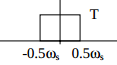
\includegraphics[width=0.2\textwidth]{figs/c3p32.png}
\label{fig:c3p32}
\end{figure} 

\begin{itemize}
\item Let $x(t) = 1 + cos(15\pi t)$ and T = 0.1 sec.
Draw $|X_s(\omega)|$ where $x_s(t) = x(t)p(t)$. 
Determine the expression for y(t).
\end{itemize} 

\subsection*{Solution}

First we calculate $X(\omega)$.

\begin{equation*}
\begin{aligned}
X(\omega) &= \pi [ 2 \delta(\omega) + 
	\delta(\omega - 15\pi) + \delta(\omega + 15 \pi)] 
\end{aligned}
\end{equation*} 

The plot of the magintude of $X(\omega)$ is:
\zcodemat{sources/c3p6a1.m}{Plot of Magnitude}

\begin{figure}[H]
\caption{Magnitude $|X(\omega)|$}
\centering
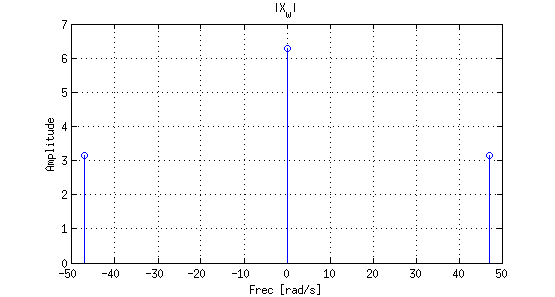
\includegraphics[width=0.8\textwidth]{figs/c3p6a1.png}
\label{fig:c3p6a1}
\end{figure} 

The minimum sampling period of the signal according to the Nyquist theorem is:

\begin{equation*}
\begin{aligned}
\omega_m &= 15 \pi \\
\omega_{Ns} >&= 2 \omega_m >= 30 \pi \\
T_{Ns} &= \frac{2 \pi}{\omega_s} <= \frac{1}{15} <= 0.066
\end{aligned}
\end{equation*} 

Since $T_s = 0.1 sec$ is greater than the minimum required,
aliasing will occur as can be seen in (\ref{fig:c3p6a2}).

\begin{equation*}
\omega_s = \frac{2 \pi}{T_s} =  20 \pi
\end{equation*} 

\zcodemat{sources/c3p6a2.m}{Plot of $|X_s(\omega)|$}

\begin{figure}[H]
\caption{Sampling $|X_s(\omega)|$}
\centering
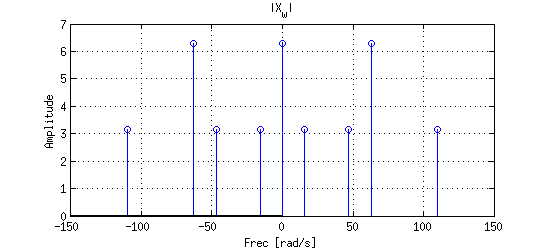
\includegraphics[width=0.8\textwidth]{figs/c3p6a2.png}
\label{fig:c3p6a2}
\end{figure}

The limits of the lowpass filter are $-0.5 \omega_s = -10 \pi$ to $0.5 \omega_s = 10 \pi$.
The Fourier transform of $Y(\omega) = H(\omega)X(\omega)$ is:

\begin{figure}[H]
\caption{Magnitude $|X(\omega)|$}
\centering
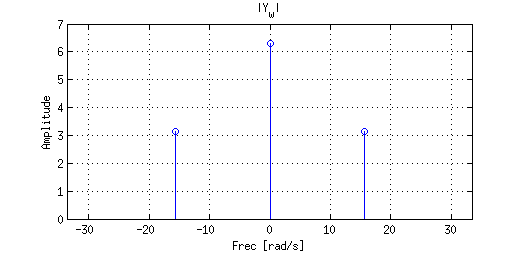
\includegraphics[width=0.8\textwidth]{figs/c3p6a3.png}
\label{fig:c3p6a3}
\end{figure}

And therefore only the $\omega = 5 \pi$ passes through it:

\begin{equation*}
\begin{aligned}
y(t) = 1 + cos(5 \pi t)
\end{aligned}
\end{equation*} 

%%%%%%%%%%%%%%%%%%%%%%%%%  B  %%%%%%%%%%%%%%%%%%%%%%%%%%%%
\begin{itemize}
\item Let $X(\omega) = \frac{1}{(j\omega+1)}$ and T = 1 sec.
Draw $|X_s(\omega)|$ where $x_s(t) = x(t)p(t)$. 
Does aliasing occur? (Justify your answer).
\end{itemize} 

\subsection*{Solution}

The magnitude of $X(\omega)$ is:
\begin{equation*}
\begin{aligned}
|X(\omega)| = \frac{1}{\omega^2 + 1}
\end{aligned}
\end{equation*} 

From the previous equation we can see that the function never intesects the w axis,
and therefore there will always be aliasing. 
However, setting $w_m$ to its FWHM we have:

\begin{equation*}
\begin{aligned}
\frac{1}{\omega_m^2+1} &= \frac{1}{2} \\
\omega_m = \sqrt{3}
\end{aligned}
\end{equation*} 

Hipoteticaly taking this value as $w_m$ we see that 
$w_s = 2 \pi > 2 w_m = 2 \sqrt{3} $ and in this case there will
not be aliasing.

The plot of the magintude of $X(\omega)$ and $X_s(\omega)$ is:
\zcodemat{sources/c3p6b1.m}{Plot of Magnitude}

\begin{figure}[H]
\caption{Magnitude}
\centering
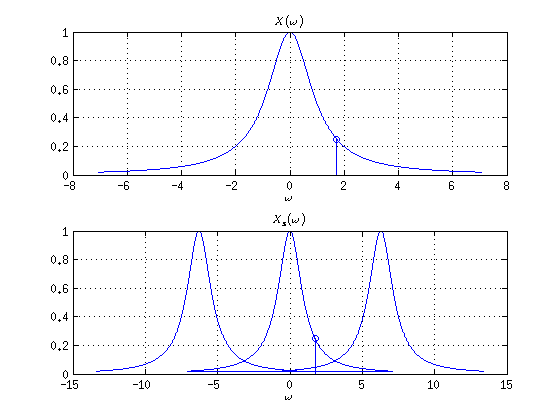
\includegraphics[width=0.8\textwidth]{figs/c3p6b2.png}
\label{fig:c3p6b2}
\end{figure} 


 
	\chapter{DTFT and DFT}
    \label{ch:dft}
    The frequency spectrum is a complex-valued function of the frequency variable, 
and thus it is usually specified in terms of an amplitude spectrum and a phase spectrum 
\cite{kamen2000fundamentals}. The complex exponential form is given by:

\begin{equation}
\begin{aligned}
x(t) &= \displaystyle\sum_{- \infty}^{\infty} X_n e^{j n \omega_0 t} \\
X_n &= \displaystyle\int_{-T/2}^{T/2} x(t) e^{-j n \omega_0 t} \; dt 
\label{eq:c11}
\end{aligned}
\end{equation}

In the next exercises we will also be using the first and/or the second 
derivative of the previous expressions (\ref{eq:c1p11}), and therefore
we write them here explicitly:

\begin{equation}
\begin{aligned}
\dot{x}(t) &= \displaystyle\sum_{- \infty}^{\infty} j n \omega_0 X_n e^{j n \omega_0 t} \\
j n \omega_0 X_n &= \displaystyle\int_{-T/2}^{T/2} \dot{x}(t) e^{-j n \omega_0 t} \; dt 
\label{eq:c12}
\end{aligned}
\end{equation}

\begin{equation}
\begin{aligned}
\ddot{x}(t) &= \displaystyle\sum_{- \infty}^{\infty} - n^2 \omega_0^2 X_n e^{j n \omega_0 t} \\
-n^2 \omega_0^2 X_n &= \displaystyle\int_{-T/2}^{T/2} \dot{x}(t) e^{-j n \omega_0 t} \; dt 
\label{eq:c13}
\end{aligned}
\end{equation}


    For each signal, find the Fourier transform, $X(\omega)$, and then plot $|X(\omega)|$ 
(note, you may want to use MATLAB for the plot in 3.)

\section*{Problem 1}

\begin{figure}[H]
\caption*{}
\centering
\includegraphics[width=0.4\textwidth]{figs/c2p11.png}
\label{fig:}
\end{figure} 

\subsection*{Solution}
Taking the derivative of $x(t)$ we get:

\begin{figure}[H]
\caption{Derivative $\dot{x}$}
\centering
\includegraphics[width=0.6\textwidth]{figs/c2p1dotx.png}
\label{fig:}
\end{figure}

Applying \ref{eq:c21} and \ref{eq:c22c} to $\dot{x}$ we have:

\begin{equation*}
\begin{aligned}
j \omega X(\omega) &= 2 \int_{-\infty}^\infty (\delta(t) - \delta(t-2))e^{-j \omega t} \; dt\\
&= 2 [ 1 - e^{-2 j \omega}] \\
&= 2 e^{-j \omega}[ e^{- j \omega} - e^{- j \omega}] \\
&= 4 j e^{-j \omega} \sin(\omega) \\
X(\omega) &= 4 \frac{\sin(\omega) }{\omega} e^{-j \omega} \\
 &= 4 Sa(\omega) e^{- j \omega}
\end{aligned}
\end{equation*} 

The plot of the magintude and angle of $X(\omega)$ is:
\zcodemat{sources/c2p1a.m}{Plot of Magnitude and Angle}

\begin{figure}[H]
\caption{Magnitude $|X(\omega)|$ and Angle}
\centering
\includegraphics[width=1.0\textwidth]{figs/c2p1a.png}
\label{fig:c2p1a}
\end{figure} 


	
	\chapter{Z-Transform}
    \label{ch:zt}

	\chapter{Haar Base}
    \label{ch:hb}
    For each signal, find the Fourier transform, $X(\omega)$, and then plot $|X(\omega)|$ 
(note, you may want to use MATLAB for the plot in 3.)

\section*{Problem 1}

\begin{figure}[H]
\caption*{}
\centering
\includegraphics[width=0.4\textwidth]{figs/c2p11.png}
\label{fig:}
\end{figure} 

\subsection*{Solution}
Taking the derivative of $x(t)$ we get:

\begin{figure}[H]
\caption{Derivative $\dot{x}$}
\centering
\includegraphics[width=0.6\textwidth]{figs/c2p1dotx.png}
\label{fig:}
\end{figure}

Applying \ref{eq:c21} and \ref{eq:c22c} to $\dot{x}$ we have:

\begin{equation*}
\begin{aligned}
j \omega X(\omega) &= 2 \int_{-\infty}^\infty (\delta(t) - \delta(t-2))e^{-j \omega t} \; dt\\
&= 2 [ 1 - e^{-2 j \omega}] \\
&= 2 e^{-j \omega}[ e^{- j \omega} - e^{- j \omega}] \\
&= 4 j e^{-j \omega} \sin(\omega) \\
X(\omega) &= 4 \frac{\sin(\omega) }{\omega} e^{-j \omega} \\
 &= 4 Sa(\omega) e^{- j \omega}
\end{aligned}
\end{equation*} 

The plot of the magintude and angle of $X(\omega)$ is:
\zcodemat{sources/c2p1a.m}{Plot of Magnitude and Angle}

\begin{figure}[H]
\caption{Magnitude $|X(\omega)|$ and Angle}
\centering
\includegraphics[width=1.0\textwidth]{figs/c2p1a.png}
\label{fig:c2p1a}
\end{figure} 



    \chapter{Haar Transform}
    \label{ch:ht}

    \bibliographystyle{plain}
    \bibliography{biblio}

\end{document}
